\chapter{Algoritmi greedy}

\index{algoritmi greedy}

Un \key{algoritmo greedy} (avido, ingordo)
costruisce una soluzione del problema
scegliendo in ogni momento quella che è 
la migliore soluzione possibile.
In questo modo
non tornano mai indietro per modificare le proprie scelte,
ma costruisco direttamente la soluzione finale.
Per questa ragione gli algoritmi greedy sono solitamente
molto efficienti.

La difficoltà nel progettare gli algoritmi greedy
è quella di trovare una strategia greedy che garantisca 
di produrre sempre la soluzione ottimale del problema.

Una scelta ottima \textit{locale} deve sempre 
essere anche una scelta che garantisce un ottimo \textit{globale},
ma spesso è difficile dimostrare che un algoritmo greedy
funziona per ogni input.


\section{Problema delle monete}

Come primo esempio si consideri il problema 
in cui viene dato un insieme di monete e lo scopo
è quello di formare una somma $n$ usando le monete date.
I valori delle monete sono
$\texttt{coins}=\{c_1,c_2,\ldots,c_k\}$,
e ogni moneta può essere usata quante volte si vuole.
Qual è il mimino numero di monete necessario per ottenere la somma richiesta?

Per esempio, se le monete fossero degli euro (espressi in centesimi)
\[\{1,2,5,10,20,50,100,200\}\]
e $n=520$,
ci sarebbe bisogno di almeno quattro monete
e la soluzione ottima sarebbe
$200+200+100+20$, la cui somma è 520.

\subsubsection{Algoritmo greedy}

Un semplice algoritmo greedy che risolve il problema 
prevede di scegliere a ogni passo la più grande moneta possibile,
fino a che la somma delle monete non sia stata raggiunta.
Questo algoritmo funziona nel caso di esempio,
perchè inizialmente si sceglie due volte la moneta da 200,
poi una volta quella da 100 e infine una da 20.
Ma questo algoritmo funziona in ogni caso?
Si può verificare che se le monete sono quelle dell'insieme
proposto, l'algoritmo funziona sempre, cioè produce sempre 
una soluzione con il più piccolo numero possibile di monete.
La correttezza dell'algoritmo può essere dimostrata in questo modo:
ognuna delle monete 1, 5, 10, 50 e 100 appaiono al massimo 
una sola volta in una soluzione ottima,
perchè, se la soluzione contenesse due di tali monete,
queste potrebbero essere rimpiazzate da una sola moneta,
ottenendo così una soluzione migliore.
Per esempio, se la soluzione contenesse $5+5$,
le due monete dovrebbero essere rimpiazzate da una moneta da $10$.

Nello stesso modo, le monete 2 e 20 possono apparire al massimo due 
volte in una soluzione ottima, perchè la somma $2+2+2$ potrebbe essere
rimpiazzata dalla somma $5+1$ e la somma $20+20+20$ potrebbe essere rimpiazzata
dalla somma $50+10$.
Inoltre una soluzione ottima non può contenere le somme
$2+2+1$ o $20+20+10$ perchè potrebbero essere 
rimpiazzate rispettivamente dalle
monete $5$ e $50$.

Usando queste osservazioni 
si può mostrare che per ogni moneta di valore $x$,
non è possibile costruire una somma ottima $x$ o maggiore di $x$
usando solo monete di valore minore di $x$.
Per esempio, se $n=100$, la migliore somma ottima possibile
usando valori minori di 100 è $50+20+20+5+2+2=99$.
Quindi l'algoritmo greedy che seleziona ad ogni passo la più
grande moneta possibile produrrà sempre una soluzione ottima.

Questo esempio dimostra che può essere difficile
dimostrare la correttezza dell'algoritmo in tutte le situazioni,
anche se l'algoritmo in sé è semplice. 

\subsubsection{Caso generale}
Il caso generale di questo esempio può contenere monete
di qualsiasi valore e l'algoritmo greedy \emph{non} porta necessariamente
a una soluzione ottima.

Si può dimostrare che il procedimento greedy non sempre
funziona mostrando un controesempio in cui si ottiene un risultato non corretto.
Per questo problema trovare un controesempio è facile:
se le monete sono hanno valori $\{1,3,4\}$ e la somma richiesta è 6,
l'algoritmo greedy produrrebbe la soluzione 
$4+1+1$, mentre è evidente che la soluzione ottima è $3+3$.

Non si sa se il caso generale del problema delle monete
possa essere risolto da un qualsiasi algoritmo greedy\footnote{Comunque è possibile
\emph{verificare} in tempo polinomiale
se l'algoritmo greedy presentato in questo capitolo
funziona per un dato insieme di monete\cite{pea05}.}.

Comunque, come si vedrà nel Capitolo 7,
in alcuni casi il problema generale può essere risolto
in maniera efficiente usando la programmazione dinamica,
che fornisce sempre la risposta corretta.

\section{Scheduling}

Molti problemi di \emph{scheduling} possono essere risolti
usando degli algoritmi greedy.
Un problema classico è il seguente:
dati $n$ eventi con i propri tempi di inizio e di fine,
trovare una sequenza che contenga il numero maggiore possibile
di eventi non sovrapposti, cioè che non contenga una o più 
coppie di eventi la cui intersezione non sia vuota.
Si condiderino ad esempio i seguenti eventi:
\begin{center}
\begin{tabular}{lll}
evento & inizio & fine \\
\hline
$A$ & 1 & 3 \\
$B$ & 2 & 5 \\
$C$ & 3 & 9 \\
$D$ & 6 & 8 \\
\end{tabular}
\end{center}
In questo caso il numero massimo di eventi è due.
Per esempio si possono selezionare gli eventi $B$ e $D$
come segue:
\begin{center}
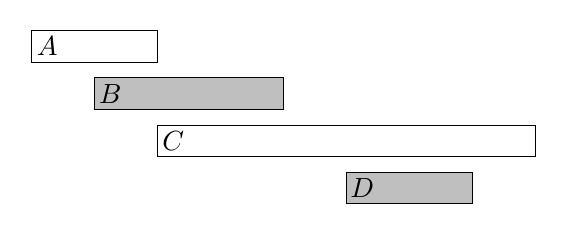
\begin{tikzpicture}[scale=.4]
  \begin{scope}
    \draw (2, 0) rectangle (6, -1);
    \draw[fill=lightgray] (4, -1.5) rectangle (10, -2.5);
    \draw (6, -3) rectangle (18, -4);
    \draw[fill=lightgray] (12, -4.5) rectangle (16, -5.5);
    \node at (2.5,-0.5) {$A$};
    \node at (4.5,-2) {$B$};
    \node at (6.5,-3.5) {$C$};
    \node at (12.5,-5) {$D$};
  \end{scope}
\end{tikzpicture}
\end{center}

Si possono inventare diversi algoritmi greedy per risolvere
questo problema, ma quale funzionerà con qualsiasi input?

\subsubsection*{Algoritmo 1}

La prima idea potrebbe essere quella di selezionare gli eventi
più \emph{corti} possibili, cioè quelli che durano di meno.
In questo esempio verrebbero selezionati i seguenti eventi:
\begin{center}
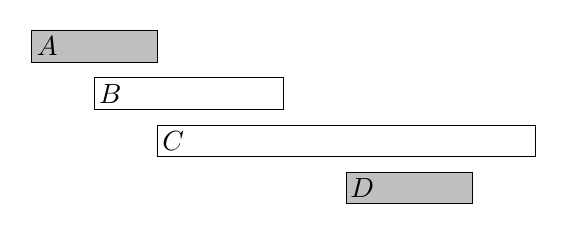
\begin{tikzpicture}[scale=.4]
  \begin{scope}
    \draw[fill=lightgray] (2, 0) rectangle (6, -1);
    \draw (4, -1.5) rectangle (10, -2.5);
    \draw (6, -3) rectangle (18, -4);
    \draw[fill=lightgray] (12, -4.5) rectangle (16, -5.5);
    \node at (2.5,-0.5) {$A$};
    \node at (4.5,-2) {$B$};
    \node at (6.5,-3.5) {$C$};
    \node at (12.5,-5) {$D$};
  \end{scope}
\end{tikzpicture}
\end{center}

Comunque questa strategia non porta sempre alla soluzione ottima.
Per esempio l'algoritmo fallisce con questi eventi:
\begin{center}
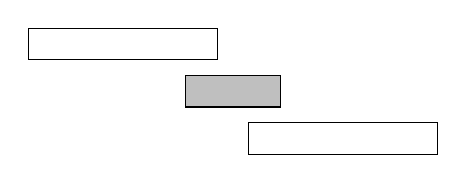
\begin{tikzpicture}[scale=.4]
  \begin{scope}
    \draw (1, 0) rectangle (7, -1);
    \draw[fill=lightgray] (6, -1.5) rectangle (9, -2.5);
    \draw (8, -3) rectangle (14, -4);
  \end{scope}
\end{tikzpicture}
\end{center}
Se viene selezionato l'evento più corto, risulta possibile selezionare solo quello,
dove la soluzione ottima prevede invece che sia possibile selezionare entrambi gli eventi più lunghi.

\subsubsection*{Algoritmo 2}

Un'altra idea potrebbe essere quella di selezionare
il prossimo evento che \emph{inizia} il \emph{prima} possibile.

Questo algoritmo seleziona i seguenti eventi:
\begin{center}
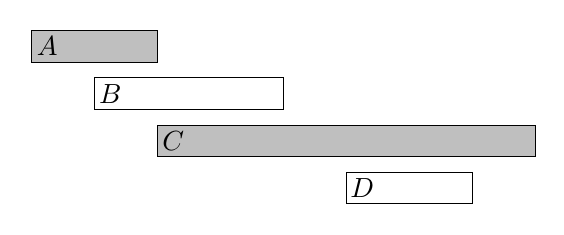
\begin{tikzpicture}[scale=.4]
  \begin{scope}
    \draw[fill=lightgray] (2, 0) rectangle (6, -1);
    \draw (4, -1.5) rectangle (10, -2.5);
    \draw[fill=lightgray] (6, -3) rectangle (18, -4);
    \draw (12, -4.5) rectangle (16, -5.5);
    \node at (2.5,-0.5) {$A$};
    \node at (4.5,-2) {$B$};
    \node at (6.5,-3.5) {$C$};
    \node at (12.5,-5) {$D$};
  \end{scope}
\end{tikzpicture}
\end{center}
 
Si riesce comunque a trovare un controesempio anche 
per questo algoritmo.
Ad esempio, per i seguenti valori,
l'algoritmo seleziona un solo evento:
\begin{center}
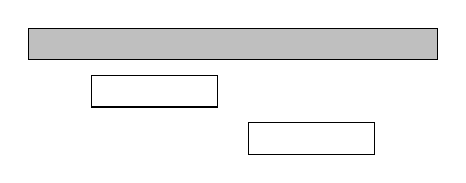
\begin{tikzpicture}[scale=.4]
  \begin{scope}
    \draw[fill=lightgray] (1, 0) rectangle (14, -1);
    \draw (3, -1.5) rectangle (7, -2.5);
    \draw (8, -3) rectangle (12, -4);
  \end{scope}
\end{tikzpicture}
\end{center}
Selezionando il primo evento non è poi possibile
selezionarne nessun altro, dove invece la soluzione ottima
contiene due eventi.

\subsubsection*{Algoritmo 3}

La terza idea è quella di selezionare il prossimo 
evento che \emph{finisce} il \emph{prima} possibile.

Questo algoritmo seleziona i seguenti eventi:
\begin{center}
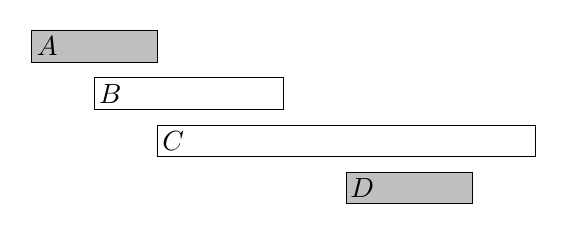
\begin{tikzpicture}[scale=.4]
  \begin{scope}
    \draw[fill=lightgray] (2, 0) rectangle (6, -1);
    \draw (4, -1.5) rectangle (10, -2.5);
    \draw (6, -3) rectangle (18, -4);
    \draw[fill=lightgray] (12, -4.5) rectangle (16, -5.5);
    \node at (2.5,-0.5) {$A$};
    \node at (4.5,-2) {$B$};
    \node at (6.5,-3.5) {$C$};
    \node at (12.5,-5) {$D$};
  \end{scope}
\end{tikzpicture}
\end{center}

Si può dimostrare che questo algoritmo produce
\emph{sempre} una soluzione ottimale.
Il motivo per cui funziona è che selezionare l'evento 
che termina per primo è una scelta ottima anche
globalmente.
Se successivamente si seleziona il prossimo evento
scegliendo quello che termina per primo tra quelli rimasti
si arriva ancora a una scelta ottima globale e continuando 
così fino a quando non si possono selezionare ulteriori eventi
si arriva alla soluzione ottima.

Un modo per dimostrare che l'algoritmo funziona
è di considerare cosa succede se al posto di selezionare
l'evento che finisce il prima possibile se 
ne seleziona uno che finisce dopo.
In questo caso il numero di ulteriori scelte possibili
non può che essere uguale o minore a quelle che si sarebbero
ottenute selezionando l'evento che termina per primo
e quindi non si potrà ottenere una soluzione migliore,
quindi questo algoritmo greedy è corretto.

\section{Attività e deadline}

Si consideri ora un problema dove siano 
date $n$ attività, ognuna con una durata e una deadline\footnote{Una data entro la quale
l'attività deve necessariamente terminare}, e il problema 
è quello di scegliere un ordine in cui eseguire le attività, una di seguito all'altra.
Inoltre per ogni attività si guadagnano $d-x$ punti,
dove $d$ è la deadline dell'attività e 
$x$ è il momento effettivo in cui si conclude l'attività,
quindi si guadagnano più punti quanto più un'attività si conclude
prima della propria deadline.
Qual è il punteggio massimo che si può ottenere 
ordinando al meglio le attività?
Si supponga ad esempio che le attività siano le seguenti:
\begin{center}
\begin{tabular}{lll}
attività & durata & deadline \\
\hline
$A$ & 4 & 2 \\
$B$ & 3 & 5 \\
$C$ & 2 & 7 \\
$D$ & 4 & 5 \\
\end{tabular}
\end{center}
In questo caso una pianificazione ottimale per le attività 
sarebbe la seguente:
\begin{center}
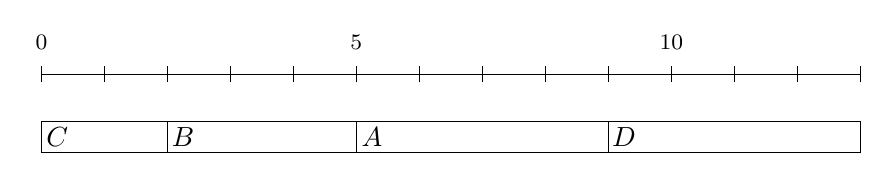
\begin{tikzpicture}[scale=.4]
  \begin{scope}
    \draw (0, 0) rectangle (4, -1);
    \draw (4, 0) rectangle (10, -1);
    \draw (10, 0) rectangle (18, -1);
    \draw (18, 0) rectangle (26, -1);
    \node at (0.5,-0.5) {$C$};
    \node at (4.5,-0.5) {$B$};
    \node at (10.5,-0.5) {$A$};
    \node at (18.5,-0.5) {$D$};

    \draw (0,1.5) -- (26,1.5);
    \foreach \i in {0,2,...,26}
    {
        \draw (\i,1.25) -- (\i,1.75);
    }
    \footnotesize
    \node at (0,2.5) {0};
    \node at (10,2.5) {5};
    \node at (20,2.5) {10};

  \end{scope}
\end{tikzpicture}
\end{center}
In questa soluzione $C$ permette di guadagnare 5 punti,
$B$ fa guadagnare 0 punti, $A$ fa perdere $-7$ punti
e $D$ altri $-8$ punti,
così che il punteggio totale finale risulta di $-10$.

Sorprendentemente la soluzione ottima non dipende affatto
dalle deadline, ma la strategia greedy corretta è semplicemente
quella di eseguire le attività \emph{ordinate per durata} in
ordine crescente.
Il motivo per cui questa strategia funziona è che
se, dati due soli task, li si ordina in modo tale che
il primo task dura più del secondo,
sicuramente si può ottenere una soluzione migliore scambiandoli,
come si può vedere dal seguente esempio:
\begin{center}
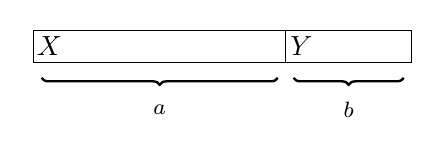
\begin{tikzpicture}[scale=.4]
  \begin{scope}
    \draw (0, 0) rectangle (8, -1);
    \draw (8, 0) rectangle (12, -1);
    \node at (0.5,-0.5) {$X$};
    \node at (8.5,-0.5) {$Y$};

\draw [decoration={brace}, decorate, line width=0.3mm] (7.75,-1.5) -- (0.25,-1.5);
\draw [decoration={brace}, decorate, line width=0.3mm] (11.75,-1.5) -- (8.25,-1.5);

\footnotesize
\node at (4,-2.5) {$a$};
\node at (10,-2.5) {$b$};

  \end{scope}
\end{tikzpicture}
\end{center}
Siccome $a>b$, si può scambiare l'ordine dell'attività:
\begin{center}
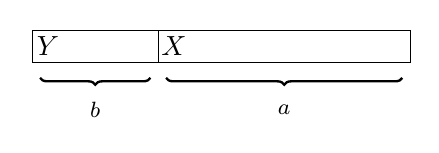
\begin{tikzpicture}[scale=.4]
  \begin{scope}
    \draw (0, 0) rectangle (4, -1);
    \draw (4, 0) rectangle (12, -1);
    \node at (0.5,-0.5) {$Y$};
    \node at (4.5,-0.5) {$X$};

\draw [decoration={brace}, decorate, line width=0.3mm] (3.75,-1.5) -- (0.25,-1.5);
\draw [decoration={brace}, decorate, line width=0.3mm] (11.75,-1.5) -- (4.25,-1.5);

\footnotesize
\node at (2,-2.5) {$b$};
\node at (8,-2.5) {$a$};

  \end{scope}
\end{tikzpicture}
\end{center}
Ora $X$ da $b$ punti in meno rispetto al primo ordinamento, ma $Y$ da $a$ punti in più,
così che il punteggio totale aumenta di $a-b > 0$.
In una soluzione ottima, date due qualsiasi attività consecutive,
deve sempre essere vero che quella più breve compaia prima di quella
più lunga, portando quindi alla conclusione che le attività debbano essere
ordinate per durata dalla più breve alla più lunga.

\section{Minimizzazione di somme}

Si consideri ora un problema dove vengano
dati $n$ numeri $a_1,a_2,\ldots,a_n$
e lo scopo sia quello di trovare un valore $x$
che minimizzi la somma
\[|a_1-x|^c+|a_2-x|^c+\cdots+|a_n-x|^c.\]
Nel seguito si analizzeranno i casi in cui $c=1$ e $c=2$.

\subsubsection{Caso $c=1$}

In questo caso l'espressione da minimizzare diventa
\[|a_1-x|+|a_2-x|+\cdots+|a_n-x|.\]
Per esempio, se i numeri fossero $[1,2,9,2,6]$,
la soluzione sarebbe $x=2$,
poichè produce la somma
\[
|1-2|+|2-2|+|9-2|+|2-2|+|6-2|=12.
\]
Nel caso generale, la scelta migliore per $x$
è il valore \textit{mediano} dei numeri,
cioè il numero che si trova nella posizione 
centrale se gli elementi vengono ordinati.
Per esempio la lista $[1,2,9,2,6]$
diventa $[1,2,2,6,9]$ dopo l'ordinamento e
il mediano è il numero 2.

Il mediano è la scelta ottimale
perchè, se $x$ fosse più piccolo del mediano
facendolo aumentare la somma diminuirebbe e,
allo stesso modo, se $x$ fosse più grande del mediano,
facendolo dimunuire la somma diminuirebbe.
Quindi il valore della somma minore si ottiene
quando $x$ è proprio il valore mediano.
Se il numero $n$ di elementi della lista fosse pari, 
si avrebbero due mediani, e quindi qualsiasi valere compreso
tra di essi (estremi inclusi), sarebbe
una scelta ottimale.

\subsubsection{Caso $c=2$}

In questo caso si dovrebbe minimizzare la somma
\[(a_1-x)^2+(a_2-x)^2+\cdots+(a_n-x)^2.\]
Se i numeri fossero, per esempio, $[1,2,9,2,6]$,
la migliore soluzione sarebbe $x=4$
che produrrebbe 46 come somma
\[
(1-4)^2+(2-4)^2+(9-4)^2+(2-4)^2+(6-4)^2=46.
\]
Nel caso generale la scelta migliore per $x$
è la \emph{media} dei numeri.
Nell'esempio precedente la media è $(1+2+9+2+6)/5=4$.
Questo risultato può essere dedotto presentando 
la somma nel seguente modo:
\[
nx^2 - 2x(a_1+a_2+\cdots+a_n) + (a_1^2+a_2^2+\cdots+a_n^2)
\]
L'ultima parte non dipende da $x$,
così può essere ignorata.
La parte rimanente è una funzione della forma
$nx^2-2xs$ dove $s=a_1+a_2+\cdots+a_n$.
Come si può vedere questa è una parabola con la concavità
verso l'alto e le sue radici sono
$x=0$ e $x=2s/n$,
e il valore minore lo assume nella media delle radici, 
che vale $x=s/n$, che è appunto la media dei numeri
$a_1,a_2,\ldots,a_n$.

\section{Data compression}

\index{data compression}
\index{binary code}
\index{codeword}

A \key{binary code} assigns for each character
of a string a \key{codeword} that consists of bits.
We can \emph{compress} the string using the binary code
by replacing each character by the
corresponding codeword.
For example, the following binary code
assigns codewords for characters
\texttt{A}–\texttt{D}:
\begin{center}
\begin{tabular}{rr}
character & codeword \\
\hline
\texttt{A} & 00 \\
\texttt{B} & 01 \\
\texttt{C} & 10 \\
\texttt{D} & 11 \\
\end{tabular}
\end{center}
This is a \key{constant-length} code
which means that the length of each
codeword is the same.
For example, we can compress the string
\texttt{AABACDACA} as follows:
\[00\,00\,01\,00\,10\,11\,00\,10\,00\]
Using this code, the length of the compressed
string is 18 bits.
However, we can compress the string better
if we use a \key{variable-length} code
where codewords may have different lengths.
Then we can give short codewords for
characters that appear often
and long codewords for characters
that appear rarely.
It turns out that an \key{optimal} code
for the above string is as follows:
\begin{center}
\begin{tabular}{rr}
character & codeword \\
\hline
\texttt{A} & 0 \\
\texttt{B} & 110 \\
\texttt{C} & 10 \\
\texttt{D} & 111 \\
\end{tabular}
\end{center}
An optimal code produces a compressed string
that is as short as possible.
In this case, the compressed string using
the optimal code is
\[0\,0\,110\,0\,10\,111\,0\,10\,0,\]
so only 15 bits are needed instead of 18 bits.
Thus, thanks to a better code it was possible to
save 3 bits in the compressed string.

We require that no codeword
is a prefix of another codeword.
For example, it is not allowed that a code
would contain both codewords 10
and 1011.
The reason for this is that we want
to be able to generate the original string
from the compressed string.
If a codeword could be a prefix of another codeword,
this would not always be possible.
For example, the following code is \emph{not} valid:
\begin{center}
\begin{tabular}{rr}
character & codeword \\
\hline
\texttt{A} & 10 \\
\texttt{B} & 11 \\
\texttt{C} & 1011 \\
\texttt{D} & 111 \\
\end{tabular}
\end{center}
Using this code, it would not be possible to know
if the compressed string 1011 corresponds to
the string \texttt{AB} or the string \texttt{C}.

\index{Huffman coding}

\subsubsection{Huffman coding}

\key{Huffman coding}\footnote{D. A. Huffman discovered this method
when solving a university course assignment
and published the algorithm in 1952 \cite{huf52}.} is a greedy algorithm
that constructs an optimal code for
compressing a given string.
The algorithm builds a binary tree
based on the frequencies of the characters
in the string,
and each character's codeword can be read
by following a path from the root to
the corresponding node.
A move to the left corresponds to bit 0,
and a move to the right corresponds to bit 1.

Initially, each character of the string is
represented by a node whose weight is the
number of times the character occurs in the string.
Then at each step two nodes with minimum weights
are combined by creating
a new node whose weight is the sum of the weights
of the original nodes.
The process continues until all nodes have been combined.

Next we will see how Huffman coding creates
the optimal code for the string
\texttt{AABACDACA}.
Initially, there are four nodes that correspond
to the characters of the string:

\begin{center}
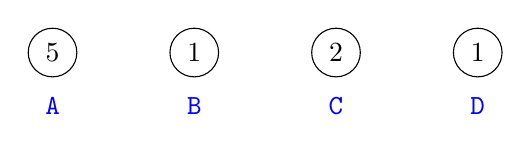
\begin{tikzpicture}[scale=0.9]
\node[draw, circle] (1) at (0,0) {$5$};
\node[draw, circle] (2) at (2,0) {$1$};
\node[draw, circle] (3) at (4,0) {$2$};
\node[draw, circle] (4) at (6,0) {$1$};

\node[color=blue] at (0,-0.75) {\texttt{A}};
\node[color=blue] at (2,-0.75) {\texttt{B}};
\node[color=blue] at (4,-0.75) {\texttt{C}};
\node[color=blue] at (6,-0.75) {\texttt{D}};

%\path[draw,thick,-] (4) -- (5);
\end{tikzpicture}
\end{center}
The node that represents character \texttt{A}
has weight 5 because character \texttt{A}
appears 5 times in the string.
The other weights have been calculated
in the same way.

The first step is to combine the nodes that
correspond to characters \texttt{B} and \texttt{D},
both with weight 1.
The result is:
\begin{center}
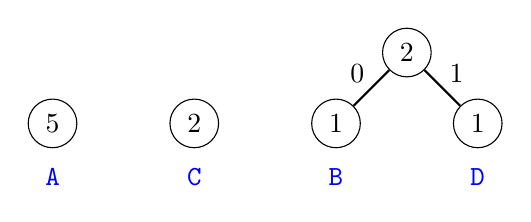
\begin{tikzpicture}[scale=0.9]
\node[draw, circle] (1) at (0,0) {$5$};
\node[draw, circle] (3) at (2,0) {$2$};
\node[draw, circle] (2) at (4,0) {$1$};
\node[draw, circle] (4) at (6,0) {$1$};
\node[draw, circle] (5) at (5,1) {$2$};

\node[color=blue] at (0,-0.75) {\texttt{A}};
\node[color=blue] at (2,-0.75) {\texttt{C}};
\node[color=blue] at (4,-0.75) {\texttt{B}};
\node[color=blue] at (6,-0.75) {\texttt{D}};

\node at (4.3,0.7) {0};
\node at (5.7,0.7) {1};

\path[draw,thick,-] (2) -- (5);
\path[draw,thick,-] (4) -- (5);
\end{tikzpicture}
\end{center}
After this, the nodes with weight 2 are combined:
\begin{center}
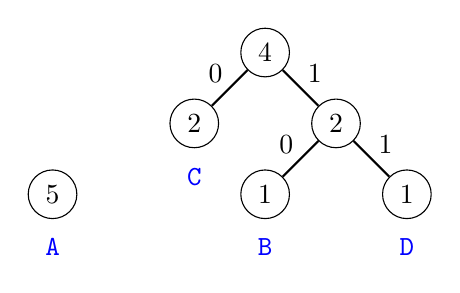
\begin{tikzpicture}[scale=0.9]
\node[draw, circle] (1) at (1,0) {$5$};
\node[draw, circle] (3) at (3,1) {$2$};
\node[draw, circle] (2) at (4,0) {$1$};
\node[draw, circle] (4) at (6,0) {$1$};
\node[draw, circle] (5) at (5,1) {$2$};
\node[draw, circle] (6) at (4,2) {$4$};

\node[color=blue] at (1,-0.75) {\texttt{A}};
\node[color=blue] at (3,1-0.75) {\texttt{C}};
\node[color=blue] at (4,-0.75) {\texttt{B}};
\node[color=blue] at (6,-0.75) {\texttt{D}};

\node at (4.3,0.7) {0};
\node at (5.7,0.7) {1};
\node at (3.3,1.7) {0};
\node at (4.7,1.7) {1};

\path[draw,thick,-] (2) -- (5);
\path[draw,thick,-] (4) -- (5);
\path[draw,thick,-] (3) -- (6);
\path[draw,thick,-] (5) -- (6);
\end{tikzpicture}
\end{center}
Finally, the two remaining nodes are combined:
\begin{center}
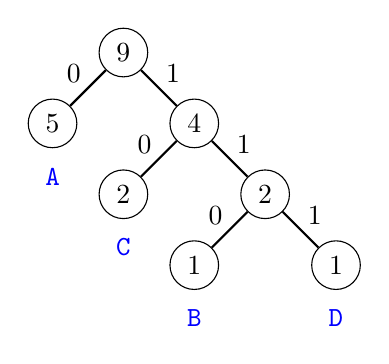
\begin{tikzpicture}[scale=0.9]
\node[draw, circle] (1) at (2,2) {$5$};
\node[draw, circle] (3) at (3,1) {$2$};
\node[draw, circle] (2) at (4,0) {$1$};
\node[draw, circle] (4) at (6,0) {$1$};
\node[draw, circle] (5) at (5,1) {$2$};
\node[draw, circle] (6) at (4,2) {$4$};
\node[draw, circle] (7) at (3,3) {$9$};

\node[color=blue] at (2,2-0.75) {\texttt{A}};
\node[color=blue] at (3,1-0.75) {\texttt{C}};
\node[color=blue] at (4,-0.75) {\texttt{B}};
\node[color=blue] at (6,-0.75) {\texttt{D}};

\node at (4.3,0.7) {0};
\node at (5.7,0.7) {1};
\node at (3.3,1.7) {0};
\node at (4.7,1.7) {1};
\node at (2.3,2.7) {0};
\node at (3.7,2.7) {1};

\path[draw,thick,-] (2) -- (5);
\path[draw,thick,-] (4) -- (5);
\path[draw,thick,-] (3) -- (6);
\path[draw,thick,-] (5) -- (6);
\path[draw,thick,-] (1) -- (7);
\path[draw,thick,-] (6) -- (7);
\end{tikzpicture}
\end{center}

Now all nodes are in the tree, so the code is ready.
The following codewords can be read from the tree:
\begin{center}
\begin{tabular}{rr}
character & codeword \\
\hline
\texttt{A} & 0 \\
\texttt{B} & 110 \\
\texttt{C} & 10 \\
\texttt{D} & 111 \\
\end{tabular}
\end{center}